% Options for packages loaded elsewhere
\PassOptionsToPackage{unicode}{hyperref}
\PassOptionsToPackage{hyphens}{url}
%
\documentclass[
]{article}
\usepackage{lmodern}
\usepackage{amssymb,amsmath}
\usepackage{ifxetex,ifluatex}
\ifnum 0\ifxetex 1\fi\ifluatex 1\fi=0 % if pdftex
  \usepackage[T1]{fontenc}
  \usepackage[utf8]{inputenc}
  \usepackage{textcomp} % provide euro and other symbols
\else % if luatex or xetex
  \usepackage{unicode-math}
  \defaultfontfeatures{Scale=MatchLowercase}
  \defaultfontfeatures[\rmfamily]{Ligatures=TeX,Scale=1}
\fi
% Use upquote if available, for straight quotes in verbatim environments
\IfFileExists{upquote.sty}{\usepackage{upquote}}{}
\IfFileExists{microtype.sty}{% use microtype if available
  \usepackage[]{microtype}
  \UseMicrotypeSet[protrusion]{basicmath} % disable protrusion for tt fonts
}{}
\makeatletter
\@ifundefined{KOMAClassName}{% if non-KOMA class
  \IfFileExists{parskip.sty}{%
    \usepackage{parskip}
  }{% else
    \setlength{\parindent}{0pt}
    \setlength{\parskip}{6pt plus 2pt minus 1pt}}
}{% if KOMA class
  \KOMAoptions{parskip=half}}
\makeatother
\usepackage{xcolor}
\IfFileExists{xurl.sty}{\usepackage{xurl}}{} % add URL line breaks if available
\IfFileExists{bookmark.sty}{\usepackage{bookmark}}{\usepackage{hyperref}}
\hypersetup{
  pdftitle={Coding to code::proof: Practice fundamentals of automated tests for collaborative data analysis development},
  pdfauthor={Charles T. Gray, IMeRG; Elise Gould, IMeRG; David Wilkinson, QAEG; Aaron Willcox, IMeRG},
  hidelinks,
  pdfcreator={LaTeX via pandoc}}
\urlstyle{same} % disable monospaced font for URLs
\usepackage[margin=1in]{geometry}
\usepackage{color}
\usepackage{fancyvrb}
\newcommand{\VerbBar}{|}
\newcommand{\VERB}{\Verb[commandchars=\\\{\}]}
\DefineVerbatimEnvironment{Highlighting}{Verbatim}{commandchars=\\\{\}}
% Add ',fontsize=\small' for more characters per line
\usepackage{framed}
\definecolor{shadecolor}{RGB}{248,248,248}
\newenvironment{Shaded}{\begin{snugshade}}{\end{snugshade}}
\newcommand{\AlertTok}[1]{\textcolor[rgb]{0.94,0.16,0.16}{#1}}
\newcommand{\AnnotationTok}[1]{\textcolor[rgb]{0.56,0.35,0.01}{\textbf{\textit{#1}}}}
\newcommand{\AttributeTok}[1]{\textcolor[rgb]{0.77,0.63,0.00}{#1}}
\newcommand{\BaseNTok}[1]{\textcolor[rgb]{0.00,0.00,0.81}{#1}}
\newcommand{\BuiltInTok}[1]{#1}
\newcommand{\CharTok}[1]{\textcolor[rgb]{0.31,0.60,0.02}{#1}}
\newcommand{\CommentTok}[1]{\textcolor[rgb]{0.56,0.35,0.01}{\textit{#1}}}
\newcommand{\CommentVarTok}[1]{\textcolor[rgb]{0.56,0.35,0.01}{\textbf{\textit{#1}}}}
\newcommand{\ConstantTok}[1]{\textcolor[rgb]{0.00,0.00,0.00}{#1}}
\newcommand{\ControlFlowTok}[1]{\textcolor[rgb]{0.13,0.29,0.53}{\textbf{#1}}}
\newcommand{\DataTypeTok}[1]{\textcolor[rgb]{0.13,0.29,0.53}{#1}}
\newcommand{\DecValTok}[1]{\textcolor[rgb]{0.00,0.00,0.81}{#1}}
\newcommand{\DocumentationTok}[1]{\textcolor[rgb]{0.56,0.35,0.01}{\textbf{\textit{#1}}}}
\newcommand{\ErrorTok}[1]{\textcolor[rgb]{0.64,0.00,0.00}{\textbf{#1}}}
\newcommand{\ExtensionTok}[1]{#1}
\newcommand{\FloatTok}[1]{\textcolor[rgb]{0.00,0.00,0.81}{#1}}
\newcommand{\FunctionTok}[1]{\textcolor[rgb]{0.00,0.00,0.00}{#1}}
\newcommand{\ImportTok}[1]{#1}
\newcommand{\InformationTok}[1]{\textcolor[rgb]{0.56,0.35,0.01}{\textbf{\textit{#1}}}}
\newcommand{\KeywordTok}[1]{\textcolor[rgb]{0.13,0.29,0.53}{\textbf{#1}}}
\newcommand{\NormalTok}[1]{#1}
\newcommand{\OperatorTok}[1]{\textcolor[rgb]{0.81,0.36,0.00}{\textbf{#1}}}
\newcommand{\OtherTok}[1]{\textcolor[rgb]{0.56,0.35,0.01}{#1}}
\newcommand{\PreprocessorTok}[1]{\textcolor[rgb]{0.56,0.35,0.01}{\textit{#1}}}
\newcommand{\RegionMarkerTok}[1]{#1}
\newcommand{\SpecialCharTok}[1]{\textcolor[rgb]{0.00,0.00,0.00}{#1}}
\newcommand{\SpecialStringTok}[1]{\textcolor[rgb]{0.31,0.60,0.02}{#1}}
\newcommand{\StringTok}[1]{\textcolor[rgb]{0.31,0.60,0.02}{#1}}
\newcommand{\VariableTok}[1]{\textcolor[rgb]{0.00,0.00,0.00}{#1}}
\newcommand{\VerbatimStringTok}[1]{\textcolor[rgb]{0.31,0.60,0.02}{#1}}
\newcommand{\WarningTok}[1]{\textcolor[rgb]{0.56,0.35,0.01}{\textbf{\textit{#1}}}}
\usepackage{graphicx}
\makeatletter
\def\maxwidth{\ifdim\Gin@nat@width>\linewidth\linewidth\else\Gin@nat@width\fi}
\def\maxheight{\ifdim\Gin@nat@height>\textheight\textheight\else\Gin@nat@height\fi}
\makeatother
% Scale images if necessary, so that they will not overflow the page
% margins by default, and it is still possible to overwrite the defaults
% using explicit options in \includegraphics[width, height, ...]{}
\setkeys{Gin}{width=\maxwidth,height=\maxheight,keepaspectratio}
% Set default figure placement to htbp
\makeatletter
\def\fps@figure{htbp}
\makeatother
\setlength{\emergencystretch}{3em} % prevent overfull lines
\providecommand{\tightlist}{%
  \setlength{\itemsep}{0pt}\setlength{\parskip}{0pt}}
\setcounter{secnumdepth}{5}
\usepackage{hyperref}
  \hypersetup{
    colorlinks=TRUE,
    citecolor=gray,
    pdftitle ={codeproof},
    linkcolor=gray,
    filecolor=gray,
    urlcolor=gray
    % bookmarks=true
    }

\newlength{\cslhangindent}
\setlength{\cslhangindent}{1.5em}
\newenvironment{cslreferences}%
  {\setlength{\parindent}{0pt}%
  \everypar{\setlength{\hangindent}{\cslhangindent}}\ignorespaces}%
  {\par}

\title{Coding to \texttt{code::proof}: Practice fundamentals of
automated tests for collaborative data analysis development}
\usepackage{etoolbox}
\makeatletter
\providecommand{\subtitle}[1]{% add subtitle to \maketitle
  \apptocmd{\@title}{\par {\large #1 \par}}{}{}
}
\makeatother
\subtitle{How to go from no tests, to \emph{whoa} tests!}
\author{Charles T. Gray, IMeRG\footnote{Special thanks to Emily Riederer
  for her ongoing correspondence throughout the writing of this
  manuscript. Thanks, also, to Hannah Fraser, Fiona Fidler, and Daniel
  Fryer. Also, appreciation for Danielle Navarro, Thomas Pedersen and
  others on twitter who helped with the visualisation.} \and Elise
Gould, IMeRG \and David Wilkinson, QAEG \and Aaron Willcox, IMeRG}
\date{}

\begin{document}
\maketitle
\begin{abstract}
Despite centuries' accumulation of pedagogy on pianistic technique,
there remains a comparative dearth of literature conceptualising the
process of obtainng sufficiant technical ability. Analogously, a
toolchain gap exists between between good enough practices of scientific
computation and implementation. A toolchain walkthrough, an opinionated
documentation of a scientific workflow, provides a means of addressing
this gap. In this toolchain walkthrough, we present a methodology for
coding to a measure of \texttt{code::proof}, a sense of good enough
confidence in the implementation of a statistical algorithm.
\end{abstract}

\newcommand{\codereg}[1]{
\fbox{\begin{minipage}{15em}
#1
\end{minipage}}
}

\hypertarget{coding-to-codeproof}{%
\section{\texorpdfstring{Coding to
\texttt{code::proof}}{Coding to code::proof}}\label{coding-to-codeproof}}

J. S. Bach's Contrapunctus I, a four-part work of counterpoint from
\emph{The Art of Fugue}, is not learnt in one sitting {[}todo:
citation{]}. Indeed, for most pianists, to play the three-minute piece
is the result of many months' diligent work, and still the piece will
never feel \emph{done}. To play well, a pianist must employ technique,
but \emph{how} a pianist is to achieve the desired technique is not
clear (Chang 2009).

For a researcher performing an analysis using a computational tool such
as R, it can be unclear when an analysis is \emph{done}. And, while
there are technical guides on \emph{good enough} practice, it can feel
overwhelming as to what to adopt and where. Particularly for an
in-development algorithm, which is to say, an algorithm with scripts
already started, and some results explored.

This manuscript picks up from where Riederer left off with
\textbf{RMarkdown-driven development} and suggests a
\texttt{code::register}ed (\texttt{c::r}ed\footnote{In this manuscript,
  \texttt{c::r} denotes \texttt{code::registration}, \texttt{c::r}ing
  denotes \texttt{code::registering}, and \texttt{c::r}ed denotes
  \texttt{code::registered}}) \textbf{test-driven workflow} for coding
to doneness. This workflow provides a roadmap to completion for a
packaged analysis with \texttt{code::proof}ed the manuscript (Gray
2019), provided measures of confidence in the implementation of the
algorithm.

Musicians and, similarly, athletes, do not see themselves as having
mastered a skill but as active practitioners of a craft (Galway 1990).
To be a flautist is to practice, and to be an athlete is to train. For
researcher developers, it can be hard to assess when an analysis is
completed. In this manuscript, we consider the \emph{practice} of
test-driven analysis development as a means of \emph{coding to doneness}
for an algorithm, a workflow that facilitates the analyst achieving
sufficient \texttt{code::proof} in their algorithm, confidence in the
implementation of the algorithm (Gray 2019).

\hypertarget{questionable-research-practices-in-scientific-computing}{%
\subsection{Questionable research practices in scientific
computing}\label{questionable-research-practices-in-scientific-computing}}

Algorithms are coded by people who \emph{practice} code, and significant
problems emerge when algorithms are treated as fixed artifacts, rather
than one of the tools utilised by those who \emph{practice} code. In
Australia, a heartbreaking ongoing example of this kind of problem is
the income-reporting data analysis algorithm that assesses if income
welfare recipients have been overpaid entitlements. Crude averaging
calculations have lead to ongoing incorrect debt notices issued, such as
20,000 people receiving ``robodebt'' notices for debts they did not owe
(McIlroy 2017). Problems in data analysis have real impacts on real
people's lives. Perhaps, if the algorithm were considered a workflow
practiced and monitored by a team of data scientists, rather than a
static object, problems would not be persisting to this day (Karp 2019).
Indeed, as noted in Wilson's testing primers (in development) for
\href{https://rstudio.cloud/learn/primers}{RStudio} (``RStudio Cloud,''
n.d.),

\begin{quote}
Almost all (92\%) of the catastrophic system failures are the result of
incorrect handling of non-fatal errors explicitly signalled in software.
In 58\% of the catastrophic failures, the underlying faults could easily
have been detected through simple testing of error handling code (Yuan
et al. 2014).
\end{quote}

We might view this as a computational instantiation of what Fraser
\emph{et al.} denote \emph{questionable research practices} (QRPs). The
QRPs Fraser \emph{et al.} provide a taxonomy for refer to various
practices in scientific methodology found in ecology and evolution, such
as \(p\)-hacking, adjusting a model's specification to achieve a desired
\(p\)-value, or \emph{cherry picking}, failing to report variables or
results that do not fit a desired narrative. QRPs are, importantly,
often not a result of scientific malpractice, but a question of
discipline-specific conventions established in bygone eras not
translating well to data-driven research (Fraser et al. 2018). In
scientific computing, as the robodebt example illustrates, similar and
overlapping errors may occur.

A consideration when providing recommendations of best practice is what
we might reasonably expect of a researcher. Indeed, it is likely
unrealistic to expect \emph{best practices} in scientific computing
(Wilson et al. 2014), perhaps we would be better off asking for
\emph{good enough} practices (Wilson et al. 2017) in scientific
computing. For while researchers use computational algorithms in science
every day, most of them are not trained in computational science. Even
mathematicians and statisticians do a great deal of training at the
blackboard, rather than the computer.

Riederer identifies several QRPs in scientific computing, for example,
hardcoded values that interfere with another's ability to reproduce the
computational results (Riederer 2019). As researcher software engineers,
it behoves us to consider what are questionable research practices in
software produced for data analyses. Version control and open code
sharing via a platform such as GitHub, is one way to mitigate
questionable research practices in scientific computing (Bryan 2017).
There is also a growing literature on reproducible research compendia
via packaged analyses (Marwick, Boettiger, and Mullen 2018; Wilson et
al. 2017).

This manuscript contributes to this literature by focussing on workflows
for using automated tests to move analysis towards a fully reproducible
packaged research compendium. Furthermore, these workflows assist the
developer to communicate what they have coded to others and their future
self, as a means of mitigating questionable research practices in
scientific computing. Above all, by providing a workflow for the
\emph{practice} of code, the developer anxiety is reduced by having the
parameters as clearly defined as they can be from the start.

\hypertarget{practice-fundamentals}{%
\subsection{Practice fundamentals}\label{practice-fundamentals}}

Chuang C. Chang's \emph{Fundamentals of Piano Practice} sets out to
address a gap in piano pedagogy (Chang 2009). A similar gap exists in
the implementation of \emph{good enough} practices (Wilson et al. 2017),
which is to say, what we might reasonably expect of an analyst, in
reproducible computing for research data analyses. The objective is
different from advanced pianism, but we characterise testing
\emph{practice}, as opposed to \emph{technique}, analogous to how Chang
delineates between \emph{piano} practice and technique. Through
attempting to identify the fundamentals of automated testing for
collaborative data analysis development, this manuscript aims to
articulate the gap in understanding automated testing implementation for
analysts.

As Chang notes, whilst there a rich history of technical pedagogy, there
is a dearth of guidance for pianists on \emph{learning} the technique
(Chang 2009). There are many canonical texts of pianistic technique
pedagogy. Bach provides a pathway from small canons {[}todo: cite{]}, to
two-part inventions {[}todo: cite{]}, three-part sinfonia, and the
challenge of \emph{The Well-Tempered Clavier} and \emph{The Art of
Fugue}. Bartok provides the \emph{Mikrokosmos} {[}todo: cite{]}, and
Czerny's \emph{School of Velocity} {[}to do: cite{]}. In each case,
technical exercises of increasing difficulty are provided. In piano
pedagogy, a \emph{technical} exercise isolates a particular aspect of
pianistic technique {[}todo examples{]}. For example, {[}todo Czerny
staccato{]}. Or, {[}todo voicing technique{]}.

The dearth that Chang attempts to address is in pianistic
\emph{practice} habits that will lead to successful adoption of these
techniques. In science, we might call this a \emph{work flow} {[}todo
cite{]}.

\begin{quote}
.. practically every piano learning method consists of showing students
what to practice, and what kinds of techniques (runs, arpeggios, legato,
staccato, trills, etc.) are needed. There are few instructions on how to
practice in order to be able to play them, which is mostly left to the
student and endless repetitions (Chang 2009).
\end{quote}

Wilson \emph{et al.} followed their work on \emph{best practices} in
scientific computing (Wilson et al. 2014), with a reflection on
\emph{good enough} practices (Wilson et al. 2017), in recognition that
we must account for what we might reasonably request of data analysis
practitioners. In this manuscript, we consider one component of
\emph{good enough} practice in data analysis: \emph{automated testing}.

Automated tests are a formalised way of implementing checks that inputs
and outputs of algorithms are as expected (Wickham 2015). Informative
messages are output that assist the developer in identifying where code
is not performing as expected.

\hypertarget{collaboration-via-automated-testing}{%
\subsection{Collaboration via automated
testing}\label{collaboration-via-automated-testing}}

At heart, automated tests are collaborative. This may be with others,
but applies at least as much to an analyst approaching their own past
work with which they have become unfamiliar, or have become anxious
about some aspect of their work. Automated tests provide an efficient
way of returning to and extending an analysis; anxiety is reduced by
having defined outcomes to explicitly code for.

Reproducible research compendia provide a means by which analysts can
share their work so that it may be extended by others, and automated
tests provide \texttt{code::proof} (Gray 2019), a measure of confidence
in the algorithm for others. Hayes expresses concern about using
algorithms published without automated tests (Hayes 2019). However, only
one quarter of the largest repository of R packages,
\href{https://cran.r-project.org/}{The Comprehensive R Archive Network},
have any automated tests (Hester 2016), highlighting that, despite
testing being identified as a `vital' part of data analysis (Wickham
2015), automated testing is yet to be widely adopted.

\hypertarget{a-toolchain-walkthrough-for-test-driven-analysis-workflow}{%
\section{A toolchain walkthrough for test-driven analysis
workflow}\label{a-toolchain-walkthrough-for-test-driven-analysis-workflow}}

From this section, we now consider the practicality of implementing
tests through a \textbf{toolchain walkthrough}, an opinionated
documentation of a scientific workflow, towards a measure of
\texttt{code::proof}, or confidence in the algorithm implementation
(Gray 2019). In particular, a toolchain walkthrough is a reflection of
\emph{one} workflow, whilst other, potentially better, workflows might
exist. This is in contrast to a comprehensive review of tools. Instead,
a toolchain walkthrough ruminates on considerations \emph{given} a set
of tools have been chosen.

Toolchain walkthroughs aim to identify obstacles and advantages in
implementation of scientific workflows. By necessity, a toolchain
walkthrough is language specific, but, ideally, observations emerge that
are useful for any appropriate language employed for data analysis, such
as Python. This toolchain walkthrough examines the \emph{process},
analogous to piano \emph{practice}, of implementing tests, as opposed to
defining comprehensively the nature of \emph{good enough} tests,
analogous to guidance on pianistic technique.

\hypertarget{objective-of-this-toolchain-walkthrough}{%
\subsection{Objective of this toolchain
walkthrough}\label{objective-of-this-toolchain-walkthrough}}

This toolchain walkthrough aims to provide guidance on implementing a
test-driven workflow for an in-development analysis. Many analyses begin
as scripts that develop {[}todo expan{]} (Riederer 2019). The central
question of this manuscript is what constitutes a minimal level of
testing for in-development analysis, where code is still being written
and features implemented. Automated tests assist in time-consuming
debugging tasks (Wickham 2015), but also in providing information for a
developer who is unfamiliar with the code (including new users
\emph{and} existing developers returning after some level of temporal
distancing).

This is a first effort in identifying the fundamentals of automated
testing for the collaborative process of developing an analysis in R.
Analogous to Riederer's \emph{RMarkdown-driven development} (Riederer
2019), which de-constructs the workflow of developing an analysis from
.Rmd notebook-style reports to packaged analyses, we consider a set a
computational tools that form a workflow to assist in the coherent
development of automated tests for data analysis. This is an extension
of the workflow suggestions provided in \emph{R Packages}, with a
specific focus on collaborative workflows in research.

\hypertarget{devops-and-assumed-expertise}{%
\subsection{Devops and assumed
expertise}\label{devops-and-assumed-expertise}}

This toolchain walkthrough assumes a knowledge of R advanced enough to
be using the language to answer scientific research claims.

\begin{itemize}
\tightlist
\item
  tools used: testthat, neet, covr
\item
  GitHub
\end{itemize}

\hypertarget{a-toolchain-walkthrough-for-cr-of}{%
\subsection{\texorpdfstring{A toolchain walkthrough for \texttt{c::r}
of\ldots{}}{A toolchain walkthrough for c::r of\ldots{}}}\label{a-toolchain-walkthrough-for-cr-of}}

This toolchain walkthrough for \texttt{c::r} reflects on the
in-development practice of code to completion on several different
research projects. Consideration of sufficient \texttt{code::proof} of
packages \texttt{varameta::} and \texttt{simeta::}, developed for the
oeuvre of doctoral work this manuscript contributes to. Another example
project is considered, The repliCATS Project software of statistical
aggregation methods, in particular \texttt{CATnap::} and
\texttt{aggreCAT::}.

For The repliCATS Project, the algorithms are not available until the
research is complete, in order to blind the other team to the
methodology. Although we cannot provide explicit code examples, the
process is considered with respect to this project, as it is an example
of collaborative in-development \texttt{c::r}.

\hypertarget{varameta}{%
\subsubsection{\texorpdfstring{\texttt{varameta::}}{varameta::}}\label{varameta}}

The \texttt{varameta::} package is in-development analysis support
software for a forthcoming manuscript, Meta-analysis of Medians.

\hypertarget{simeta}{%
\subsubsection{\texorpdfstring{\texttt{simeta::}}{simeta::}}\label{simeta}}

Words words words

\hypertarget{replicats-project}{%
\subsubsection{repliCATS Project}\label{replicats-project}}

Moar words words words

\hypertarget{neet-tests}{%
\section{\texorpdfstring{\texttt{neet::}
tests}{neet:: tests}}\label{neet-tests}}

The workflow described in this toolchain walkthrough differentiates
between \ldots{}

\hypertarget{the-neet-package}{%
\subsection{\texorpdfstring{The \texttt{neet::}
package}{The neet:: package}}\label{the-neet-package}}

\begin{Shaded}
\begin{Highlighting}[]
\KeywordTok{library}\NormalTok{(neet)}
\end{Highlighting}
\end{Shaded}

A \textbf{neet test} checks a function outputs a \textbf{non-empty}
thing of \textbf{expected type}. This is what is referred to as a
\textbf{boundary condition} test in RStudio's primers (todo: citation).

These expectations are intended to integrate into minimal testing
workflow \emph{for the development} of data analyses. When developing a
function, we will need parameters, and structure of the pipeline. These
tests enable the developer to feel reassured the pipeline's functions
are outputting non-empty things of expected type, while the developer
decides the best structure for an analysis pipeline.

A \texttt{character} string will be checked for being of string-length
\textgreater{} 1.

A \texttt{numeric} is checked for not being \texttt{NA}, \texttt{NULL},
\texttt{Inf}, or \texttt{-Inf}.

A `list`` is checked for being of length \textgreater{} 1.

A \texttt{data.frame} is checked for having at least one row.

A \texttt{ggplot} object is checked for successfully running.

\hypertarget{installation}{%
\subsection{Installation}\label{installation}}

You can install the released version of \texttt{neet} from GitHub with:

\begin{Shaded}
\begin{Highlighting}[]
\CommentTok{\# Install devtools}
\KeywordTok{install.packages}\NormalTok{(devtools) }

\CommentTok{\# Use devtools to install package from GitHub}
\NormalTok{devtools}\OperatorTok{::}\KeywordTok{install\_github}\NormalTok{(}\StringTok{"softloud/neet"}\NormalTok{)}
\end{Highlighting}
\end{Shaded}

\hypertarget{example}{%
\subsubsection{Example}\label{example}}

This is a basic example which shows you how to solve a common problem:

\begin{Shaded}
\begin{Highlighting}[]
\KeywordTok{library}\NormalTok{(testthat)}
\KeywordTok{library}\NormalTok{(neet)}

\CommentTok{\#\# Basic example code}

\CommentTok{\# Expectations check output of code in testthat files}
\KeywordTok{expect\_neet}\NormalTok{(}\DecValTok{3}\NormalTok{, }\StringTok{"numeric"}\NormalTok{) }\CommentTok{\# test numeric}
\KeywordTok{expect\_neet}\NormalTok{(}\StringTok{"cat"}\NormalTok{, }\StringTok{"character"}\NormalTok{) }\CommentTok{\# test character string}
\KeywordTok{expect\_neet}\NormalTok{(mtcars, }\StringTok{"data.frame"}\NormalTok{) }\CommentTok{\# test data frame}

\CommentTok{\# Assertions check inputs of code in function scripts}
\KeywordTok{assert\_neet}\NormalTok{(}\DecValTok{3}\NormalTok{, }\StringTok{"numeric"}\NormalTok{) }\CommentTok{\# test numeric}
\end{Highlighting}
\end{Shaded}

\begin{verbatim}
## [1] TRUE
\end{verbatim}

\begin{Shaded}
\begin{Highlighting}[]
\KeywordTok{assert\_neet}\NormalTok{(}\StringTok{"cat"}\NormalTok{, }\StringTok{"character"}\NormalTok{) }\CommentTok{\# test character string}
\end{Highlighting}
\end{Shaded}

\begin{verbatim}
## [1] TRUE
\end{verbatim}

\begin{Shaded}
\begin{Highlighting}[]
\KeywordTok{assert\_neet}\NormalTok{(mtcars, }\StringTok{"data.frame"}\NormalTok{) }\CommentTok{\# test data frame}
\end{Highlighting}
\end{Shaded}

\begin{verbatim}
## [1] TRUE
\end{verbatim}

\hypertarget{codeproof-test-driven-workflow}{%
\section{\texorpdfstring{\texttt{code::proof} test-driven
workflow}{code::proof test-driven workflow}}\label{codeproof-test-driven-workflow}}

In order to\ldots{} doneness \ldots{} propose test driven \ldots{}
implemented as\ldots{}

\begin{center}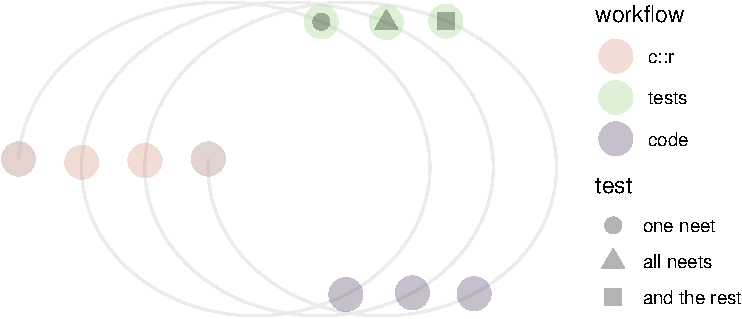
\includegraphics{when-is-done-done_files/figure-latex/unnamed-chunk-2-1} \end{center}

The model begins with a \texttt{code::registration}, an outline of the
intended algorithm, its inputs, and outputs.

A workflow includes three stages, repeated three times, before returning
to the start, the \texttt{c::r}.

Each phase consists of:

\begin{enumerate}
\def\labelenumi{\arabic{enumi}.}
\tightlist
\item
  \texttt{c::r}
\item
  tests
\item
  code
\end{enumerate}

\hypertarget{codeproof-workflow-for-coding-to-doneness}{%
\subsection{\texorpdfstring{\texttt{code::proof} workflow for coding to
doneness}{code::proof workflow for coding to doneness}}\label{codeproof-workflow-for-coding-to-doneness}}

The tests vary each time in complexity, so that the complete model cycle
consists of ten phases of work:

\begin{enumerate}
\def\labelenumi{\arabic{enumi}.}
\tightlist
\item
  \texttt{c::r}
\item
  neet tests, one per function
\item
  code
\item
  \texttt{c::r}
\item
  neet tests, for all inputs for each function
\item
  code
\item
  \texttt{c::r}
\item
  tests, and the rest, i.e., any other cases to test for
\item
  code
\item
  \texttt{c::r}
\end{enumerate}

We use \emph{model} cycle to denote the workflow may be adapted for
different use-cases. Our next section steps through each phase of work.

\hypertarget{coding-to-codeproof-toolchain-walkthrough}{%
\subsection{\texorpdfstring{Coding to \texttt{code::proof} toolchain
walkthrough}{Coding to code::proof toolchain walkthrough}}\label{coding-to-codeproof-toolchain-walkthrough}}

In this section we step through the Coding to \texttt{code::proof}
for\ldots{}

\begin{itemize}
\tightlist
\item
  \texttt{varameta::}, an in-development analysis that has seen many
  iterations.\\
\item
  \texttt{simeta::}
\item
  \texttt{repliCATS}
\end{itemize}

\hypertarget{coderegistration-cr}{%
\section{\texorpdfstring{\texttt{code::registration}
(\texttt{c::r})}{code::registration (c::r)}}\label{coderegistration-cr}}

\begin{center}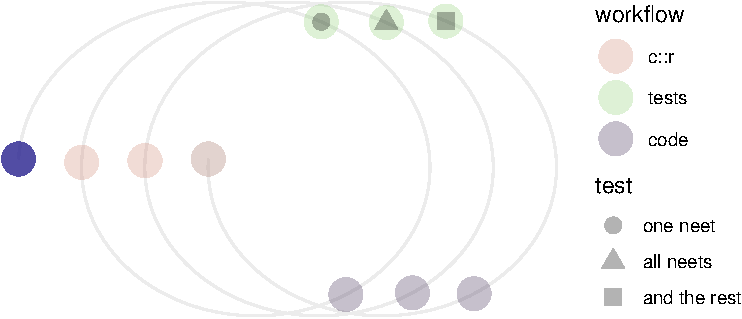
\includegraphics{when-is-done-done_files/figure-latex/unnamed-chunk-3-1} \end{center}

We begin with a sketch outline of a \texttt{code::registration}
(\texttt{c::r}), which we then populate with description in prose,
provide some detail of neet testing, before providing case-studies.

As our first testing objective is one neet test per function, we need
not necessarily work out the details of all possible things to check
for. We simply ask, what will it take to check that each function
required for the algorithm produces a non-empty thing of expected type?
For the second \texttt{code::proof} cycle, we consider all possible
inputs, and write tests, and then code for those.

The final phase, which we need not detail immediately, covers testing
for anything else we may wish to check. This might be checking there are
positive numbers output by the function. Or it might be rigorously
checking that the algorithm matches the output of another person's
instantiation of the algorithm, as is the case with the
\texttt{aggreCAT::} package.

\begin{verbatim}
1. Objective:

2. Inputs:

- [ ] one neet
- [ ] all neets
- [ ] and the rest

3. Outputs:

- [ ] one neet
- [ ] all neets
- [ ] and the rest
\end{verbatim}

Note that \texttt{-\ {[}\ {]}} will create an unchecked tickbox and
\texttt{-\ {[}x{]}} will create a tickbox in both GitHub and RMarkdown.

For the examples below, in the interest of brevity, we will drop the
tick boxes, and provide the roughly descriptive prose for the three
sections of each \texttt{c::r}. Under this workflow, we expect to update
the \texttt{c::r} as our understanding of the algorithmic structure
becomes more nuanced.

\hypertarget{varameta-cr}{%
\subsection{\texorpdfstring{\texttt{varameta::\ c::r}}{varameta:: c::r}}\label{varameta-cr}}

\begin{Shaded}
\begin{Highlighting}[]
\NormalTok{neet}\OperatorTok{::}\KeywordTok{workflow}\NormalTok{(}\DecValTok{1}\NormalTok{)}
\end{Highlighting}
\end{Shaded}

\begin{center}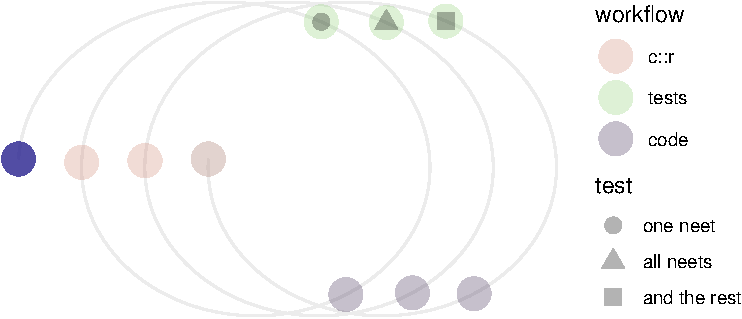
\includegraphics{when-is-done-done_files/figure-latex/unnamed-chunk-4-1} \end{center}

The \texttt{varameta::} package has the least complex structure of the
examples we are considering.

\textbf{Objective}

The \texttt{varameta::} package aims to provide a collection of
different estimators for approximating the variance of the sample
median.

\textbf{Inputs}

Each estimator takes various sample statistics (quartiles, etc.), sample
size.

\begin{itemize}
\tightlist
\item[$\square$]
  one neet
\item[$\square$]
  all neets
\item[$\square$]
  and the rest
\end{itemize}

\textbf{Outputs}

Each estimator outputs an estimate of spread and centre. Some are
approximations of the variance of the sample median, and others
approximate the standard deviation and mean.

\begin{itemize}
\tightlist
\item[$\square$]
  one neet
\item[$\square$]
  all neets
\item[$\square$]
  and the rest
\end{itemize}

\hypertarget{simeta-cr}{%
\subsection{\texorpdfstring{\texttt{simeta::\ c::r}}{simeta:: c::r}}\label{simeta-cr}}

The \texttt{simeta::} package is being developed to evaluate the
efficacy of the estimators provided in the \texttt{varameta::} package.

\textbf{Objective:}

Randomly generate meta-analysis data, calculate a confidence interval
based on a user-specified estimator (currently only works on
\texttt{varameta::}), and evaluates if the true parameter falls within;
repeat this \textbar trials\textbar{} number of times, and return the
coverage, the proportion of times the true parameter falls within the
confidence interval.

Summarise and provide a dataframe of coverage for different sample
sizes, group effect ratios, variability between studies, and
distributions. Also provide summary visualisation tools.

\begin{itemize}
\item[$\square$]
  Initial objective: provide analysis support for the meta-analysis of
  medians paper.
\item[$\square$]
  Secondary objective: allow the user to specify the estimator.
\end{itemize}

\textbf{Inputs:}

User inputs: default to \emph{just} the estimator.

\textbf{Outputs}

A dataframe of coverage probabilities.

\hypertarget{aggrecat}{%
\subsection{\texorpdfstring{\texttt{aggreCAT::}}{aggreCAT::}}\label{aggrecat}}

As the \texttt{aggreCAT::} package forms part of a pipeline of packages
designed to build a continuously integrated analysis for living data,
there are more detailed supplementary materials detailing requirements
for inputs and outputs to turn to, thus the \texttt{c::r} is somewhat
brief on first pass.

\textbf{Objective}

Provide export-ready data for each of the 19 aggregation functions.

\textbf{Inputs}

Expert judgements to be aggregated. Some special functions take other
supplementary datasets, too.

\textbf{Outputs}

A wrapper function outputs each dataset in wide client-ready format.

\hypertarget{first-cycle-one-neet-test-per-function}{%
\section{\texorpdfstring{First cycle: one \texttt{neet} test per
function}{First cycle: one neet test per function}}\label{first-cycle-one-neet-test-per-function}}

For the first \texttt{code::proof} cycle, we follow the steps:

\begin{enumerate}
\def\labelenumi{\arabic{enumi}.}
\tightlist
\item
  A rough, first-draft \texttt{c::r}.
\item
  Write one \texttt{neet} test per function.
\item
  Write code to make those \texttt{neet} tests pass, for each function.
\end{enumerate}

If functions are already written, then we only need to \emph{confirm}
the functions pass the \texttt{neet} tests.

\hypertarget{second-codeproof-cycle}{%
\section{\texorpdfstring{Second \texttt{code::proof}
cycle}{Second code::proof cycle}}\label{second-codeproof-cycle}}

\hypertarget{third-codeproof-cycle}{%
\section{\texorpdfstring{Third \texttt{code::proof}
cycle}{Third code::proof cycle}}\label{third-codeproof-cycle}}

\hypertarget{and-the-rest}{%
\subsection{And the rest}\label{and-the-rest}}

Now that we have neet tests for each function, we might ask what else
needs to be tested.

In the case of \texttt{varameta::}, we might calculate a fixed-value
output and compare it, but calculations rapidly become too complex to
calculate explicitly.

In the case of \texttt{aggreCAT::} for the repliCATS Project, we have
several aggregation methods to compare. In a large-scale collaborative
project such as this, we have several different researchers contributing
methods which the Reproducibility Team are engineering as open-source
research software. In this case, the algorithms are being
computationally implemented in software by different researchers than
those who conducted the initial analyses. And that means, with a bit of
collating, we have access to many testing datasets.

In Figure @ref(fig:aggregators), we present the results of
in-development tests on the aggregation methods developed for The
RepliCATS project.

\begin{Shaded}
\begin{Highlighting}[]
\NormalTok{knitr}\OperatorTok{::}\KeywordTok{include\_graphics}\NormalTok{(}\StringTok{"cs\_diff\_by\_method\_id.png"}\NormalTok{)}
\end{Highlighting}
\end{Shaded}

\begin{figure}

{\centering 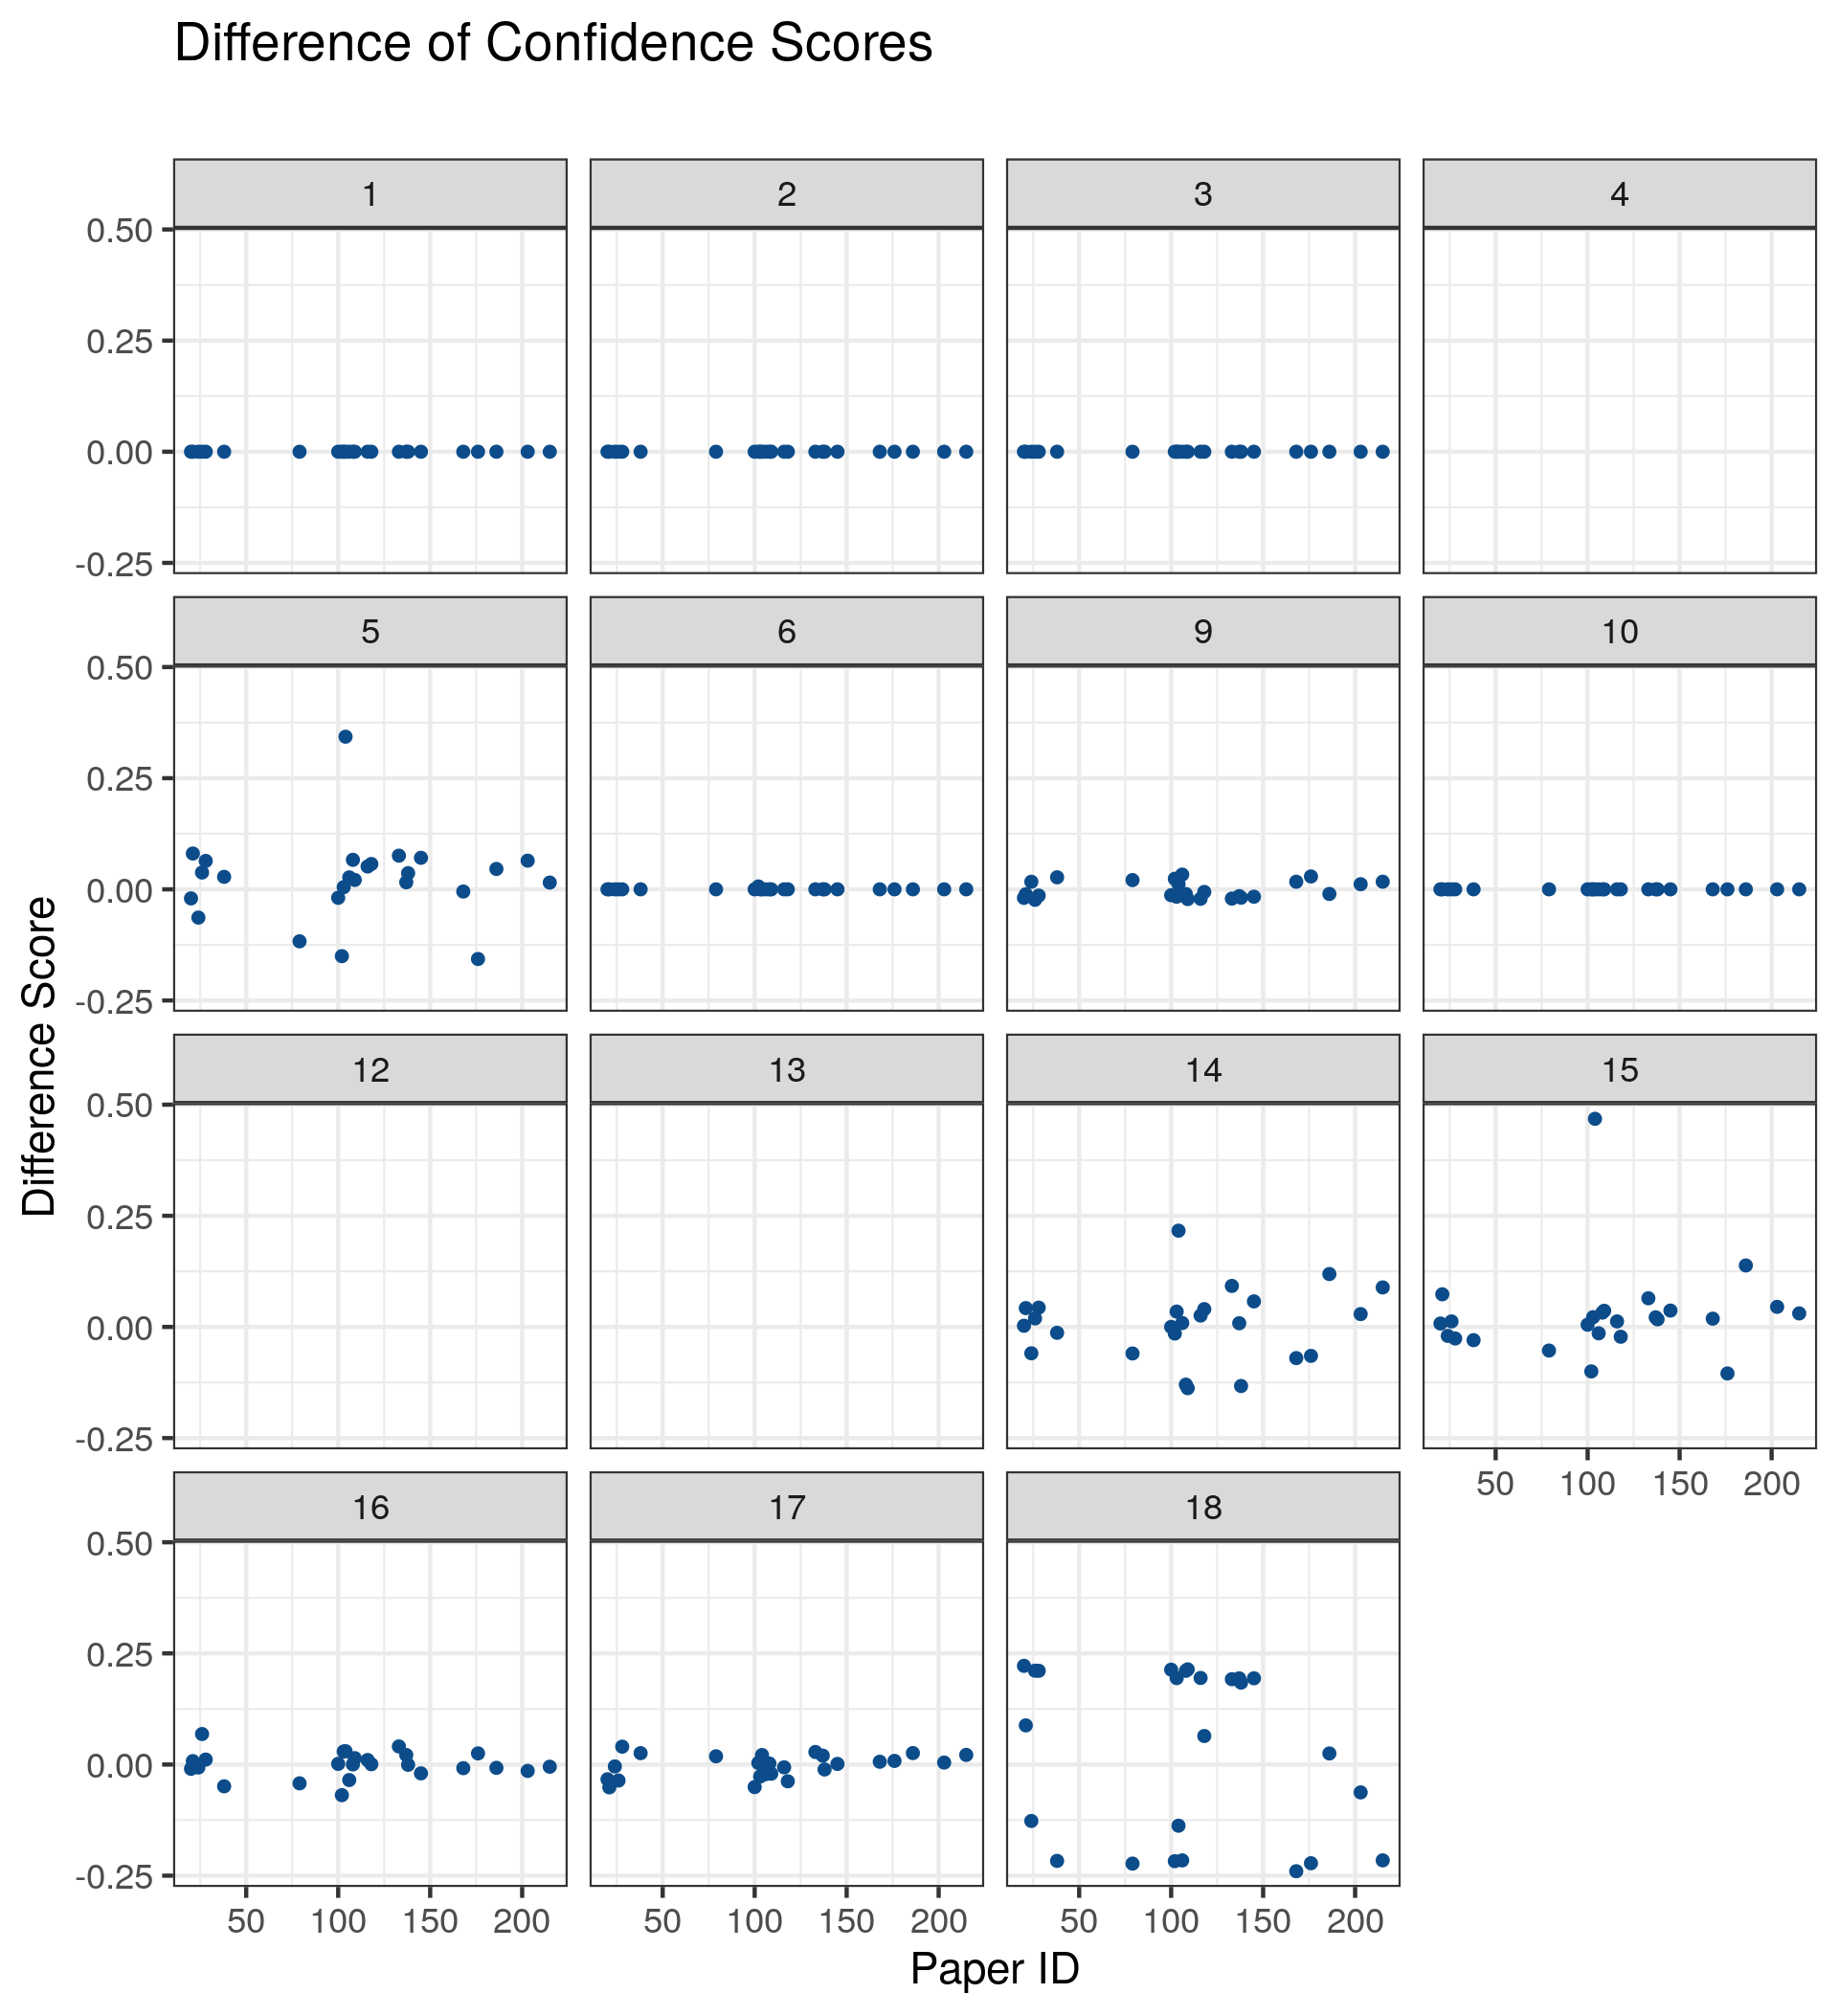
\includegraphics[width=26.68in]{cs_diff_by_method_id} 

}

\caption{\label{fig:aggregators} After neet tests are written, a comparison of aggregation methods with other researchers' analyses. Methods such as 1,6, 10, are in close agreement. There are some methods that are relatively close, such as 9 and 17. These may be deemed close enough, in consultation with the researchers who developed the methods. Then there are methods to investigate, such as 18 and 16, where there is variability between the two analyses. The aggregation methods are deidentified and the code for this visualisation will not be available until the repliCATS Project is complete, to blind the other research teams on the SCORE Program to the methods used for analysis.}\label{fig:aggregators}
\end{figure}

\hypertarget{test-coverage-with-covr}{%
\subsection{\texorpdfstring{Test coverage with
\texttt{covr::}}{Test coverage with covr::}}\label{test-coverage-with-covr}}

\begin{itemize}
\tightlist
\item
  preamble
\end{itemize}

The \texttt{covr::} function, \texttt{::package\_coverage}, provides the
percentage of the lines of code run in tests and is a succinct method to
get an at-a-glance sense coverage of testing scripts. But this assumes
we have considered everything that might require testing. Whilst this is
informative, it's not comprehensive. A \texttt{100\%} in all functions
in \texttt{covr::}, is informative, but is not done.

Consider a function that takes a number \(x\), and outputs \(2\log(x)\).
To demonstrate this we make a toy package \texttt{testtest::} comprising
this single function.

\begin{Shaded}
\begin{Highlighting}[]
\NormalTok{logfn <{-}}\StringTok{ }\ControlFlowTok{function}\NormalTok{(x) \{}
  \DecValTok{2} \OperatorTok{*}\StringTok{ }\KeywordTok{log}\NormalTok{(x)}
\NormalTok{\}}
\end{Highlighting}
\end{Shaded}

Now, we write a test that checks the function returns a numeric.

\begin{Shaded}
\begin{Highlighting}[]
\KeywordTok{library}\NormalTok{(testthat)}

\KeywordTok{test\_that}\NormalTok{(}\StringTok{"function returns numeric"}\NormalTok{, \{}
  \KeywordTok{expect\_is}\NormalTok{(}\KeywordTok{logfn}\NormalTok{(}\DecValTok{3}\NormalTok{), }\StringTok{"numeric"}\NormalTok{)}
\NormalTok{\})}
\end{Highlighting}
\end{Shaded}

And if we run \texttt{covr::package\_coverage}, we get \texttt{100\%}
for overall package coverage.

\begin{Shaded}
\begin{Highlighting}[]
\NormalTok{testtest Coverage}\OperatorTok{:}\StringTok{ }\FloatTok{100.00}\NormalTok{\%}
\NormalTok{R}\OperatorTok{/}\NormalTok{logfn.R}\OperatorTok{:}\StringTok{ }\FloatTok{100.00}\NormalTok{\%}
\end{Highlighting}
\end{Shaded}

But if we were to add this test, for negative numbers.

\begin{Shaded}
\begin{Highlighting}[]
\KeywordTok{test\_that}\NormalTok{(}\StringTok{"log function works"}\NormalTok{, \{}
  \KeywordTok{expect\_is}\NormalTok{(}\KeywordTok{logfn}\NormalTok{(}\OperatorTok{{-}}\DecValTok{1}\NormalTok{), }\StringTok{"numeric"}\NormalTok{)}
\NormalTok{\})}
\end{Highlighting}
\end{Shaded}

Then \texttt{covr::package\_coverage} fails.

\begin{Shaded}
\begin{Highlighting}[]
\OperatorTok{>}\StringTok{ }\NormalTok{covr}\OperatorTok{::}\KeywordTok{package\_coverage}\NormalTok{()}
\NormalTok{Error}\OperatorTok{:}\StringTok{ }\NormalTok{Failure }\ControlFlowTok{in} \StringTok{\textasciigrave{}}\DataTypeTok{/tmp/RtmpDjfm3d/R\_LIBS654b3cfe6ca/testtest/testtest{-}tests/testthat.Rout.fail}\StringTok{\textasciigrave{}}
\KeywordTok{library}\NormalTok{(testthat)}
\OperatorTok{>}\StringTok{ }\KeywordTok{library}\NormalTok{(testtest)}
\OperatorTok{>}\StringTok{ }
\ErrorTok{>}\StringTok{ }\KeywordTok{test\_check}\NormalTok{(}\StringTok{"testtest"}\NormalTok{)}
\NormalTok{── }\FloatTok{1.}\NormalTok{ Failure}\OperatorTok{:}\StringTok{ }\NormalTok{log }\ControlFlowTok{function} \KeywordTok{works}\NormalTok{ (}\OperatorTok{@}\NormalTok{test}\OperatorTok{{-}}\NormalTok{logfn.R}\CommentTok{\#10)  ──────────────────────────}
\KeywordTok{any}\NormalTok{(}\KeywordTok{is.na}\NormalTok{(thing\_to\_test)) isn}\StringTok{\textquotesingle{}t false.}

\StringTok{── 2. Failure: log function works (@test{-}logfn.R\#10)  ──────────────────────────}
\StringTok{any(abs(as.numeric(thing\_to\_test)) == Inf) isn\textquotesingle{}}\NormalTok{t false.}

\NormalTok{══ testthat results  ═══════════════════════════════════════════════════════════}
\NormalTok{[ OK}\OperatorTok{:}\StringTok{ }\DecValTok{8} \OperatorTok{|}\StringTok{ }\NormalTok{SKIPPED}\OperatorTok{:}\StringTok{ }\DecValTok{0} \OperatorTok{|}\StringTok{ }\NormalTok{WARNINGS}\OperatorTok{:}\StringTok{ }\DecValTok{1} \OperatorTok{|}\StringTok{ }\NormalTok{FAILED}\OperatorTok{:}\StringTok{ }\DecValTok{2}\NormalTok{ ]}
\FloatTok{1.}\NormalTok{ Failure}\OperatorTok{:}\StringTok{ }\NormalTok{log }\ControlFlowTok{function} \KeywordTok{works}\NormalTok{ (}\OperatorTok{@}\NormalTok{test}\OperatorTok{{-}}\NormalTok{logfn.R}\CommentTok{\#10) }
\FloatTok{2.}\NormalTok{ Failure}\OperatorTok{:}\StringTok{ }\NormalTok{log }\ControlFlowTok{function} \KeywordTok{works}\NormalTok{ (}\OperatorTok{@}\NormalTok{test}\OperatorTok{{-}}\NormalTok{logfn.R}\CommentTok{\#10) }

\NormalTok{Error}\OperatorTok{:}\StringTok{ }\NormalTok{testthat unit tests failed}
\NormalTok{Execution halted}
\end{Highlighting}
\end{Shaded}

\hypertarget{aggrecat-from-the-replicats-project}{%
\subsection{\texorpdfstring{\texttt{aggreCAT::} from the repliCATS
Project}{aggreCAT:: from the repliCATS Project}}\label{aggrecat-from-the-replicats-project}}

A luxury afforded in this large-scale collaborative project is that the
software implementation is implemented by different analysts than those
who developed the statistical algorithms. Different analysts developed
different algorithms, and thus, when the research software engineers on
the Reproducibility Team came to implement the algorithms there is a
wealth of pre-existing analyses to benchmark the software against.

For a small-scale analysis, the method and implementation are often
developed by one person, with minimal hands-on input from others, as is
the case with the \texttt{simeta::} and \texttt{varameta::} packages
also discussed. However, when the development and implementation are
divided between people, an opportunity for quality assurance presents
itself.

This is analogous to the quality assurance for data entry suggested by
Yenni \emph{et al.} (Yenni et al. 2019). To update a living data set,
collected in the field, the authors suggest two researchers perform the
data entry into different spreadsheets, which are then put through text
comparison algorithms to identify typos and inconsistencies.

In the case of \texttt{aggreCAT::}, there are nineteen aggregation
methods, each of which has been contributed by a researcher. Thus, each
researcher who developed a method has provided a testing dataset for the
Reproducibility Team to compare the results of the software implementing
the aggregation methods.

\hypertarget{cr-of-doneness}{%
\subsection{\texorpdfstring{\texttt{c::r} of
doneness}{c::r of doneness}}\label{cr-of-doneness}}

\begin{Shaded}
\begin{Highlighting}[]
\KeywordTok{workflow}\NormalTok{(}\DecValTok{10}\NormalTok{)}
\end{Highlighting}
\end{Shaded}

\begin{center}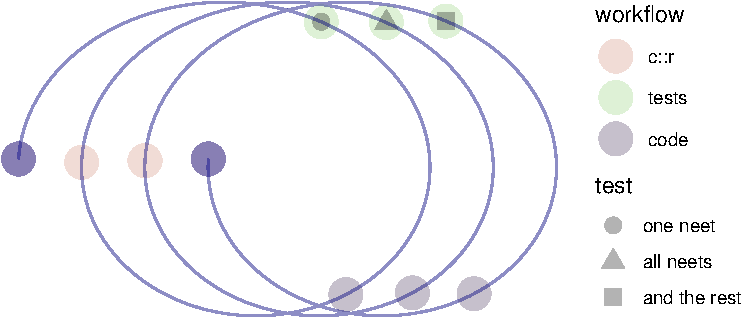
\includegraphics{when-is-done-done_files/figure-latex/unnamed-chunk-10-1} \end{center}

Under this workflow, the \texttt{c::r} is the project overview any
developer can return to. So, this final registration not only summarises
what has been tested, but also notes any idiosyncrasies for other
developers, \emph{especially} the future self of the developer who
recalls so little of the code they may as well be a different developer.

At this point, the developer makes a final assessment of whether the
stated objective of the implementation of the algorithm has been
reached. Assess the \texttt{code::proof}, through the development
process, new ideas, boundaries to check (recall the \texttt{logfn} and
negative numbers example in Section 5.4{[}todo: hyperlink{]}). We might
characterise done as when we feel we have sufficient
\texttt{code::proof}.

If the algorithm does not yet have sufficient \texttt{code::proof}, the
cycle can be repeated, and \texttt{c::r}s updates.

\hypertarget{sufficient-codeproof-of-software-for-doneness}{%
\section{\texorpdfstring{Sufficient \texttt{code::proof} of software for
doneness}{Sufficient code::proof of software for doneness}}\label{sufficient-codeproof-of-software-for-doneness}}

It does not feel a great leap to assume that we none of us will think of
every use case, every aspect, of solving an algorithm computationally.
Thus, rather than disputing what is or is not \emph{done}, we simply set
out to achieve \emph{what we can think of doing}. A \texttt{c::r}
provides a summary of what we could think of doing to `further the
process of scientific discovery', as Devezer \emph{et al.} might put it
(Devezer et al. 2019), towards our goal.

The first version of this manuscript, itself, is a pre-registration of a
computational workflow. This workflow is for \texttt{team\ reprocat::}
of the repliCATS Project to develop reproducible algorithms more happily
together. The first version provides a description of the workflow for
the team; the second version incorporates the team's feedback. This
arguably literalises the scientific practices of publishing manuscripts;
no manuscript, no matter how definitive, provides everything required
for a research project, but may offer particular tools and evidence to
further the process of scientific discovery.

Another research software engineer may be cognisant of a tool you are
unfamiliar with. By providing the package, and the \texttt{c::r}, we
provide a method to facilitate what Stodden describes as the
\emph{extensibility} of the algorithm (Stodden, Borwein, and Bailey
2013).

The workflow presented in this manuscript aims to address:
\texttt{code::xiety}, the anxiety associating with programming;
\emph{good enough} scientific practices, by incorporating automated
testing (Wilson et al. 2017); and collaborative benefits. \texttt{c::r}
provides a means of providing accessibility and transparency to the next
developer. \emph{Especially} if the next developer is your future self.

\hypertarget{older-draft}{%
\section{older draft}\label{older-draft}}

\hypertarget{get-an-overview-with-covr}{%
\subsection{\texorpdfstring{Get an overview with
\texttt{covr::}\label{sec: covr}}{Get an overview with covr::}}\label{get-an-overview-with-covr}}

For an in-development packaged analysis, the \texttt{covr::} package
provides a means of assessing the testing coverage for each function.
The analysis functions provided by \texttt{varameta::} were put on hold
while significant discussion was written for the thesis of which
\texttt{varameta::} forms a part. Beginning with
\texttt{covr::package\_coverage}, enables us to get a more informed
sense of the \texttt{code::proof} of this package, and what
\texttt{code::proof} is still required to declare the analysis done.

We pick up the long-neglected \texttt{varameta::} package at
\texttt{70\%} package coverage. But as we have seen above, this is
informative, but not completely informative. From here we examine how we
might use tests to achieve sufficient \texttt{code::proof}, confidence
in the implementation of the algorithm.

\begin{Shaded}
\begin{Highlighting}[]
\KeywordTok{library}\NormalTok{(covr)}
\KeywordTok{package\_coverage}\NormalTok{(}\StringTok{"\textasciitilde{}/Documents/repos/varameta/"}\NormalTok{)}
\CommentTok{\#> varameta Coverage: 70.71\%}
\CommentTok{\#> R/dist\_name.R: 0.00\%}
\CommentTok{\#> R/g\_cauchy.R: 44.44\%}
\CommentTok{\#> R/g\_norm.R: 71.43\%}
\CommentTok{\#> R/hozo\_se.R: 92.31\%}
\CommentTok{\#> R/bland\_mean.R: 100.00\%}
\CommentTok{\#> R/bland\_se.R: 100.00\%}
\CommentTok{\#> R/effect\_se.R: 100.00\%}
\CommentTok{\#> R/g\_exp.R: 100.00\%}
\CommentTok{\#> R/g\_lnorm.R: 100.00\%}
\CommentTok{\#> R/hozo\_mean.R: 100.00\%}
\CommentTok{\#> R/wan\_mean\_C1.R: 100.00\%}
\CommentTok{\#> R/wan\_mean\_C2.R: 100.00\%}
\CommentTok{\#> R/wan\_mean\_C3.R: 100.00\%}
\CommentTok{\#> R/wan\_se\_C1.R: 100.00\%}
\CommentTok{\#> R/wan\_se\_C2.R: 100.00\%}
\CommentTok{\#> R/wan\_se\_C3.R: 100.00\%}
\end{Highlighting}
\end{Shaded}

Created on 2020-02-01 by the \href{https://reprex.tidyverse.org}{reprex
package} (v0.3.0)

An excellent way to arrive at \emph{done} for an algorithm is to define,
even if only broadly, what \emph{done} looks like \emph{before} we set
out. We define what \texttt{code::proof} is required.

\hypertarget{code-with-intent}{%
\section{Code with intent}\label{code-with-intent}}

When we think of an algorithm, it's easy to feel overwhelmed by the
complexity. And, analogous to the pitfalls of the piano student, a
developer may fall prey to the inevitable rabbit holes and distractions
that arise. It's tempting to consider these distractions benign, but, in
fact, these actions are frequently the result of technical anxiety about
the task, and are anathema to mastering the technique in question.

\hypertarget{practice-with-intent}{%
\subsection{Practice with intent}\label{practice-with-intent}}

In learning Bach's Contrapunctus I, the student has various
conventional, albeit questionable, methods of approach.

The student might begin from the start each time. But, as the piece is
not yet mastered, the student will inevitably encounter something they
cannot play with ease. This is often encountered in the first bar of a
Bach piece. If the student plays up to the mistake, and begins again,
then they risk becoming adept the start, and becoming increasingly
anxious about the end of the piece.\\
In an advanced piece such as Contrapunctus I, there are many challenging
technical aspects. In particular, the work is polyphonic; Contrapunctus
I is a central focus of the string quartet in Vikram Seth's \emph{An
Equal Music} {[}todo citation{]}. There is a melody; formally referred
to as a \emph{subject}.

\begin{quote}
todo: figure of subject
\end{quote}

This figure reoccurs in bars\ldots.

\begin{quote}
Piano teachers know that students must practice musically in order to
acquire technique. Both musicality and technique require accuracy and
control. Practically any technical flaw can be detected in the music.
Nonetheless, many students tend to practice neglecting the music,
preferring to ``work'' when no one is around to listen. Their reasoning
is, ``I'll practice non- musically (which is easier because you can shut
off the brain) until I can play it well, then I'll add the music.'' This
never works because learning piano is all about training the brain, not
finger callisthenics (Chang 2009).
\end{quote}

\hypertarget{mindful-coding}{%
\subsection{Mindful coding}\label{mindful-coding}}

In the \texttt{varameta::} package, we wish to compare various
estimators. There are inputs, an estimator, which is to say a
computational process and a similar output, however the devil is in the
details, as

Here are the relationships between inputs, and just some of the
estimators, and outputs in \texttt{varameta}, presented as a randomised
\emph{graph}, a visual representation of a set of nodes, \(V\), and the
edges, \(V \times V\), between them. We understand each function's
inputs and outputs, but understanding the way they relate to each other,
is often muddled without planning. Our \texttt{code::brain}, the way we
conceptualise the code, is disorganised.

\begin{figure}

{\centering 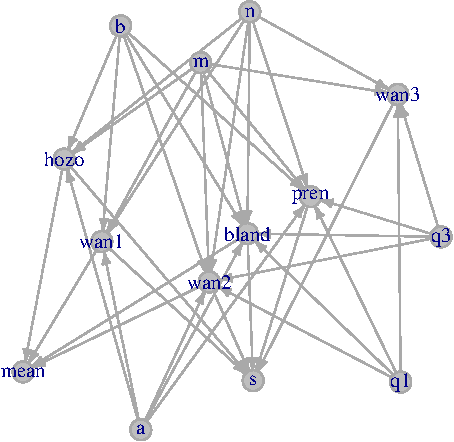
\includegraphics{when-is-done-done_files/figure-latex/codebrain-1} 

}

\caption{`code::brain` before `c::r`.}\label{fig:codebrain}
\end{figure}

\begin{verbatim}
## NULL
\end{verbatim}

The Center for Open Science recommend \emph{pre-registering} an
experiment, stating what the hypothesis is and how the analyst intends
to assess the hypothesis as one safeguard against inadvertent
questionable research practices. Analogously, we might think of
pre-registering our code as providing some \texttt{code::proof} of the
implementation of our algorithm. In this manuscript, we will think of
\emph{c::r}, stating what the intention of an algorithm is, as - todo:
complete

To code::register an algorithm:

\hypertarget{coderegistration-cr-1}{%
\section{\texorpdfstring{\texttt{code::registration\ (c::r)}}{code::registration (c::r)}}\label{coderegistration-cr-1}}

In an issue on GitHub:

\begin{enumerate}
\def\labelenumi{\arabic{enumi}.}
\tightlist
\item
  Describe the algorithm's intended purpose.
\item
  Describe the input parameters and how they will be tested.
\item
  Describe the output parameters and how they will be tested.
\end{enumerate}

Update the c::r as needed.

\hypertarget{for-complex-projects}{%
\subsection{For complex projects}\label{for-complex-projects}}

\hypertarget{on-a-piece-of-paper.}{%
\subsubsection{On a piece of paper.}\label{on-a-piece-of-paper.}}

\begin{enumerate}
\def\labelenumi{\arabic{enumi}.}
\tightlist
\item
  Draw a diagram of the inputs and outputs of the algorithm.
\item
  Draw where this algorithm fits in the pipeline of the package, if
  appropriate.
\end{enumerate}

\hypertarget{write-issue}{%
\subsubsection{Write issue}\label{write-issue}}

\begin{enumerate}
\def\labelenumi{\arabic{enumi}.}
\tightlist
\item
  Describe the algorithm's intended purpose.
\item
  Describe the input parameters and how they will be tested.
\item
  Describe the output parameters and how they will be tested.
\end{enumerate}

\hypertarget{sketch-diagram}{%
\subsubsection{Sketch-diagram}\label{sketch-diagram}}

An image or diagram is very helpful, if not burdensomely time consuming
(but it often is). This section is only useful for those who enjoy graph
theory and visualisation, and is not essential.

For those comfortable with \emph{graphs} understood as mathematical
objects as a set of vertices from \(V\), and a set of edges
\(V \times V\), there are visualisation options where the vertices can
be tagged with attributes. The code for constructing the following
\texttt{nodes} and \texttt{edges} dataframes has been omitted for
brevity, but all code can be found in this manuscript's associated
repository \href{https://github.com/softloud/neet}{\texttt{neet}} on
GitHub.

\begin{Shaded}
\begin{Highlighting}[]
\KeywordTok{library}\NormalTok{(tidyverse)}
\KeywordTok{library}\NormalTok{(ggraph)}
\KeywordTok{library}\NormalTok{(tidygraph)}
\end{Highlighting}
\end{Shaded}

By tagging the nodes in this graph with the attribute \texttt{state} in
the algorithm: starting with \texttt{input} for the estimators, sample
quartiles (which we denote \(a, q1, m, q3, b\), in order from smallest
to largest); \texttt{estimator}, a collection of functions that provide
statistical methods for preparing summary medians for meta-analysis; and
the \texttt{output} of the estimator.

\begin{Shaded}
\begin{Highlighting}[]
\NormalTok{nodes}
\end{Highlighting}
\end{Shaded}

\begin{verbatim}
## # A tibble: 24 x 2
##    node    state    
##    <chr>   <fct>    
##  1 a       input    
##  2 b       input    
##  3 q1      input    
##  4 q3      input    
##  5 m       input    
##  6 n       input    
##  7 hozo    estimator
##  8 pren_c3 estimator
##  9 pren_c1 estimator
## 10 bland   estimator
## # ... with 14 more rows
\end{verbatim}

Edges are specified by a two-column dataframe, \texttt{edges}, where
each row contains a \texttt{to} and \texttt{from} vertex identifier, the
row number of the \texttt{nodes} dataframe.

\begin{Shaded}
\begin{Highlighting}[]
\NormalTok{edges}
\end{Highlighting}
\end{Shaded}

\begin{verbatim}
## # A tibble: 84 x 2
##     from    to
##    <dbl> <dbl>
##  1     5     7
##  2     6     7
##  3     1     7
##  4     2     7
##  5     7    15
##  6     7    16
##  7     5    11
##  8     6    11
##  9     1    11
## 10     2    11
## # ... with 74 more rows
\end{verbatim}

These two dataframes can be converted into a graph object that is
compatible with the \texttt{igraph::} package and \texttt{tidyverse::}
syntax.

\begin{Shaded}
\begin{Highlighting}[]
\NormalTok{graph <{-}}\StringTok{ }\KeywordTok{tbl\_graph}\NormalTok{(nodes, edges)}
\end{Highlighting}
\end{Shaded}

These can be

\begin{Shaded}
\begin{Highlighting}[]
\NormalTok{graph }\OperatorTok{\%>\%}\StringTok{ }
\StringTok{  }\KeywordTok{mutate}\NormalTok{(}\DataTypeTok{state =} \KeywordTok{fct\_relevel}\NormalTok{(state, }\StringTok{"output"}\NormalTok{)) }\OperatorTok{\%>\%}\StringTok{ }
\StringTok{  }\KeywordTok{ggraph}\NormalTok{() }\OperatorTok{+}
\StringTok{  }\KeywordTok{geom\_edge\_link}\NormalTok{(}\DataTypeTok{arrow =} \KeywordTok{arrow}\NormalTok{(), }\DataTypeTok{colour =} \StringTok{"lightgrey"}\NormalTok{) }\OperatorTok{+}\StringTok{ }
\StringTok{  }\KeywordTok{geom\_node\_label}\NormalTok{(}\KeywordTok{aes}\NormalTok{(}\DataTypeTok{label =}\NormalTok{ node, }\DataTypeTok{colour =}\NormalTok{ state),  }
                  \DataTypeTok{size =} \DecValTok{5}\NormalTok{,}
                  \DataTypeTok{fill =} \StringTok{"lightgrey"}\NormalTok{,}
                  \DataTypeTok{alpha =} \FloatTok{0.6}\NormalTok{) }\OperatorTok{+}
\StringTok{  }\KeywordTok{theme\_graph}\NormalTok{() }\OperatorTok{+}
\StringTok{  }\NormalTok{hrbrthemes}\OperatorTok{::}\KeywordTok{scale\_color\_ipsum}\NormalTok{() }\OperatorTok{+}
\StringTok{  }\KeywordTok{theme}\NormalTok{(}\DataTypeTok{legend.position =} \StringTok{"none"}\NormalTok{,}
        \DataTypeTok{panel.background =} \KeywordTok{element\_rect}\NormalTok{(}\DataTypeTok{colour =} \StringTok{"\#ffffe0"}\NormalTok{),}
        \DataTypeTok{plot.background =} \KeywordTok{element\_rect}\NormalTok{(}\DataTypeTok{colour =} \StringTok{"\#ffffe0"}\NormalTok{)) }\OperatorTok{+}\StringTok{ }
\StringTok{  }\KeywordTok{scale\_y\_reverse}\NormalTok{() }\OperatorTok{+}\StringTok{ }
\StringTok{  }\KeywordTok{coord\_flip}\NormalTok{()}
\end{Highlighting}
\end{Shaded}

\begin{figure}

{\centering 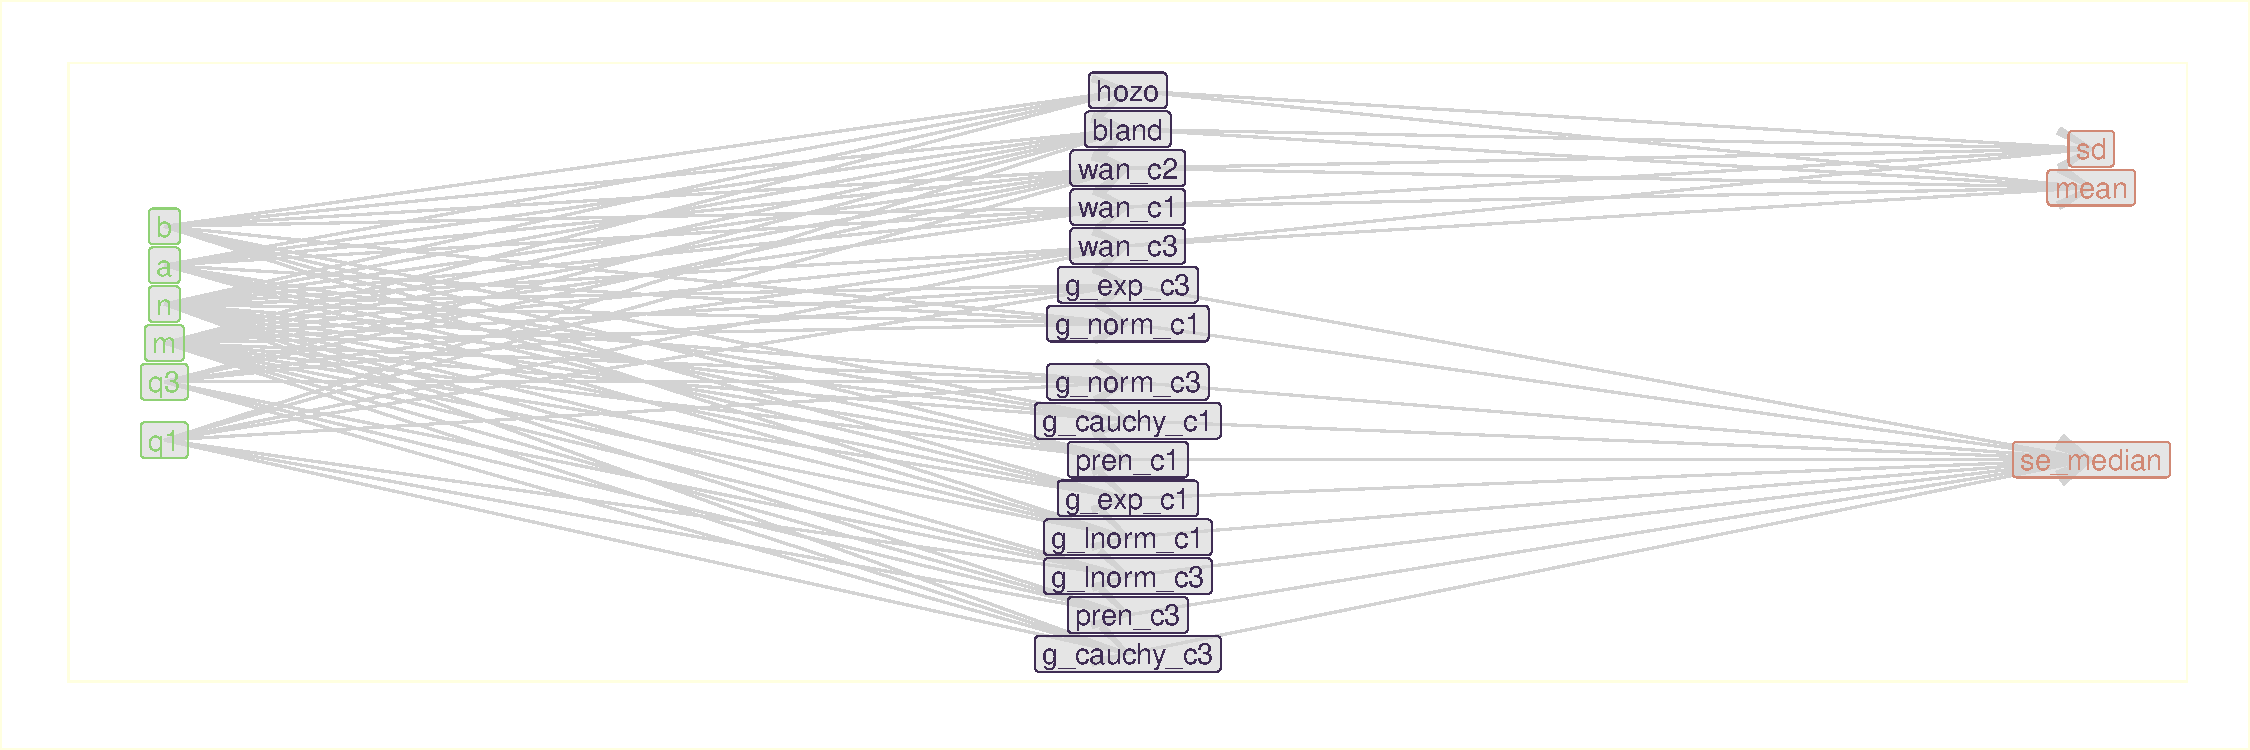
\includegraphics{when-is-done-done_files/figure-latex/unnamed-chunk-14-1} 

}

\caption{`code::brain` after `c::r`.}\label{fig:unnamed-chunk-14}
\end{figure}

\hypertarget{workflow-for-algorithmic-structure}{%
\section{Workflow for algorithmic
structure}\label{workflow-for-algorithmic-structure}}

\begin{itemize}
\tightlist
\item
  hard to find ap lace t ostart
\end{itemize}

The \texttt{neet::} package is part of this manuscript's research
compendia, we think of compendia, a collection of components that form a
research project. In the case of this manuscript, there is an extension
package of \texttt{testthat::}.

\begin{Shaded}
\begin{Highlighting}[]
\CommentTok{\# install devtools}
\KeywordTok{install.packages}\NormalTok{(devtools) }

\CommentTok{\# use devtools to install package from github}
\NormalTok{devtools}\OperatorTok{::}\KeywordTok{install\_github}\NormalTok{(}\StringTok{"softloud/neet"}\NormalTok{)}
\end{Highlighting}
\end{Shaded}

\hypertarget{references}{%
\section*{References}\label{references}}
\addcontentsline{toc}{section}{References}

\hypertarget{refs}{}
\begin{cslreferences}
\leavevmode\hypertarget{ref-Bryan2017ExcuseMD}{}%
Bryan, Jennifer. 2017. ``Excuse Me, Do You Have a Moment to Talk About
Version Control?'' \emph{PeerJ PrePrints} 5: e3159.

\leavevmode\hypertarget{ref-chang_fundamentalspianopractice_2009a}{}%
Chang, Chuan C. 2009. \emph{Fundamentals of Piano Practice}.

\leavevmode\hypertarget{ref-devezerScientificDiscoveryModelcentric2019}{}%
Devezer, Berna, Luis G. Nardin, Bert Baumgaertner, and Erkan Ozge
Buzbas. 2019. ``Scientific Discovery in a Model-Centric Framework:
Reproducibility, Innovation, and Epistemic Diversity.'' \emph{PLOS ONE}
14 (5): e0216125. \url{https://doi.org/10.1371/journal.pone.0216125}.

\leavevmode\hypertarget{ref-fraser_questionable_2018}{}%
Fraser, Hannah, Tim Parker, Shinichi Nakagawa, Ashley Barnett, and Fiona
Fidler. 2018. ``Questionable Research Practices in Ecology and
Evolution.'' \emph{PLOS ONE} 13 (7): e0200303.
\url{https://doi.org/10.1371/journal.pone.0200303}.

\leavevmode\hypertarget{ref-galway_flute_1990}{}%
Galway, James. 1990. \emph{Flute}. Kahn \& Averill.

\leavevmode\hypertarget{ref-grayCodeProofPrepare2019}{}%
Gray, Charles T. 2019. ``Code::Proof: Prepare for Most Weather
Conditions.'' In \emph{Statistics and Data Science}, edited by Hien
Nguyen, 22--41. Communications in Computer and Information Science.
Singapore: Springer. \url{https://doi.org/10.1007/978-981-15-1960-4_2}.

\leavevmode\hypertarget{ref-hayes_testing_2019}{}%
Hayes, Alex. 2019. ``Testing Statistical Software - Aleatoric.'' Blog.

\leavevmode\hypertarget{ref-hester_covr_2016}{}%
Hester, Jim. 2016. ``Covr: Bringing Test Coverage to R.''

\leavevmode\hypertarget{ref-karp_robodebtfederalcourt_2019}{}%
Karp, Paul. 2019. ``Robodebt: The Federal Court Ruling and What It Means
for Targeted Welfare Recipients.'' \emph{The Guardian}, November.

\leavevmode\hypertarget{ref-marwick_packaging_2018}{}%
Marwick, Ben, Carl Boettiger, and Lincoln Mullen. 2018. ``Packaging Data
Analytical Work Reproducibly Using R (and Friends).'' e3192v2. PeerJ
Inc. \url{https://doi.org/10.7287/peerj.preprints.3192v2}.

\leavevmode\hypertarget{ref-mcilroy201720}{}%
McIlroy, T. 2017. ``20,000 People Sent Centrelink `Robo-Debt' Notices
Found to Owe Less or Nothing.'' \emph{Canberra Times} 13.

\leavevmode\hypertarget{ref-riederer_rmarkdowndrivendevelopment_2019}{}%
Riederer, Emily. 2019. ``RMarkdown Driven Development (RmdDD).''
\emph{Emily Riederer}.

\leavevmode\hypertarget{ref-_rstudiocloud_}{}%
``RStudio Cloud.'' n.d. https://rstudio.cloud/learn/primers.

\leavevmode\hypertarget{ref-stodden_setting_2013}{}%
Stodden, Victoria, Jonathan Borwein, and David H. Bailey. 2013.
``"Setting the Default to Reproducible'' in Computational Science
Research.'' \emph{SIAM News} 46 (5).

\leavevmode\hypertarget{ref-wickham_r_2015}{}%
Wickham, H. 2015. \emph{R Packages: Organize, Test, Document, and Share
Your Code}. O'Reilly Media.

\leavevmode\hypertarget{ref-wilson_best_2014}{}%
Wilson, Greg, D. A. Aruliah, C. Titus Brown, Neil P. Chue Hong, Matt
Davis, Richard T. Guy, Steven H. D. Haddock, et al. 2014. ``Best
Practices for Scientific Computing.'' Edited by Jonathan A. Eisen.
\emph{PLoS Biology} 12 (1): e1001745.
\url{https://doi.org/10.1371/journal.pbio.1001745}.

\leavevmode\hypertarget{ref-wilson_good_2017}{}%
Wilson, Greg, Jennifer Bryan, Karen Cranston, Justin Kitzes, Lex
Nederbragt, and Tracy K. Teal. 2017. ``Good Enough Practices in
Scientific Computing.'' Edited by Francis Ouellette. \emph{PLOS
Computational Biology} 13 (6): e1005510.
\url{https://doi.org/10.1371/journal.pcbi.1005510}.

\leavevmode\hypertarget{ref-yenni_developingmoderndata_2019}{}%
Yenni, Glenda M., Erica M. Christensen, Ellen K. Bledsoe, Sarah R. Supp,
Renata M. Diaz, Ethan P. White, and S. K. Morgan Ernest. 2019.
``Developing a Modern Data Workflow for Regularly Updated Data.''
\emph{PLOS Biology} 17 (1): e3000125.
\url{https://doi.org/10.1371/journal.pbio.3000125}.

\leavevmode\hypertarget{ref-yuan_simpletestingcan_2014}{}%
Yuan, Ding, Yu Luo, Xin Zhuang, Guilherme Renna Rodrigues, Xu Zhao,
Yongle Zhang, Pranay U. Jain, and Michael Stumm. 2014. ``Simple Testing
Can Prevent Most Critical Failures: An Analysis of Production Failures
in Distributed Data-Intensive Systems.'' In \emph{Proceedings of the
11th USENIX Conference on Operating Systems Design and Implementation},
249--65. OSDI'14. Broomfield, CO: USENIX Association.
\end{cslreferences}

\end{document}
